\subsection{Hardwarekonzept}
  Das Hardwarekonzept des Dojos ist in der Abbildung \ref{fig:HWKonzept} dargestellt. 
  Man erkennt, dass es sich um ein System mit einem Mikrocontroller (nRF832) und diversen Hilfsbausteinen handelt. Es wird der nRF52832 verwendet, weil dieser eine BLE-fähige Peripherie beinhaltet und somit weiter bluetoothspezifische Hardware entfällt. 
  Ein Teil der restlichen Elektronik kümmert sich um die Energie. Mittels einer Ladeschaltung wird der Akkumulator geladen, falls der Dojo über USB eingesteckt ist und der Energieversorgungsblock erzeugt aus der Akkumulatorspannung die Arbeitsspannung der restlichen Schaltung. Auf die Energieversorgung wird im Kapitel \ref{sec:Energie} detailliert eingegangen.
  Damit Sounddateien auf dem Dojo abgespeichert werden können, beinhaltet dieser eine SD-Karte. Für das Übertragen der Dateien über USB ist die USB-SDIO-Bridge zuständig (siehe Kapitel \ref{sec:USB}).
  Das Abspielen der Sounddateien erfolgt über den Soundmanager-Block, welcher den WTV020 beinhaltet und über den nachfolgenden Treiber. Dieses Teilsystem ist im Kapitel \ref{sec:AUDIO} genauer beschrieben.
  Da sowohl der USB- als auch der Sound-Teil auf die SD-Karte zugreifen, muss ein Multiplexer verwendet werden (siehe Kapitel \ref{sec:SD_KART}). 
  Die restliche Hardware besteht aus Ein- und Ausgaben, die vom nRF52 fast direkt angesteuert werden.
  
  \begin{figure}[ht]
    \centering
    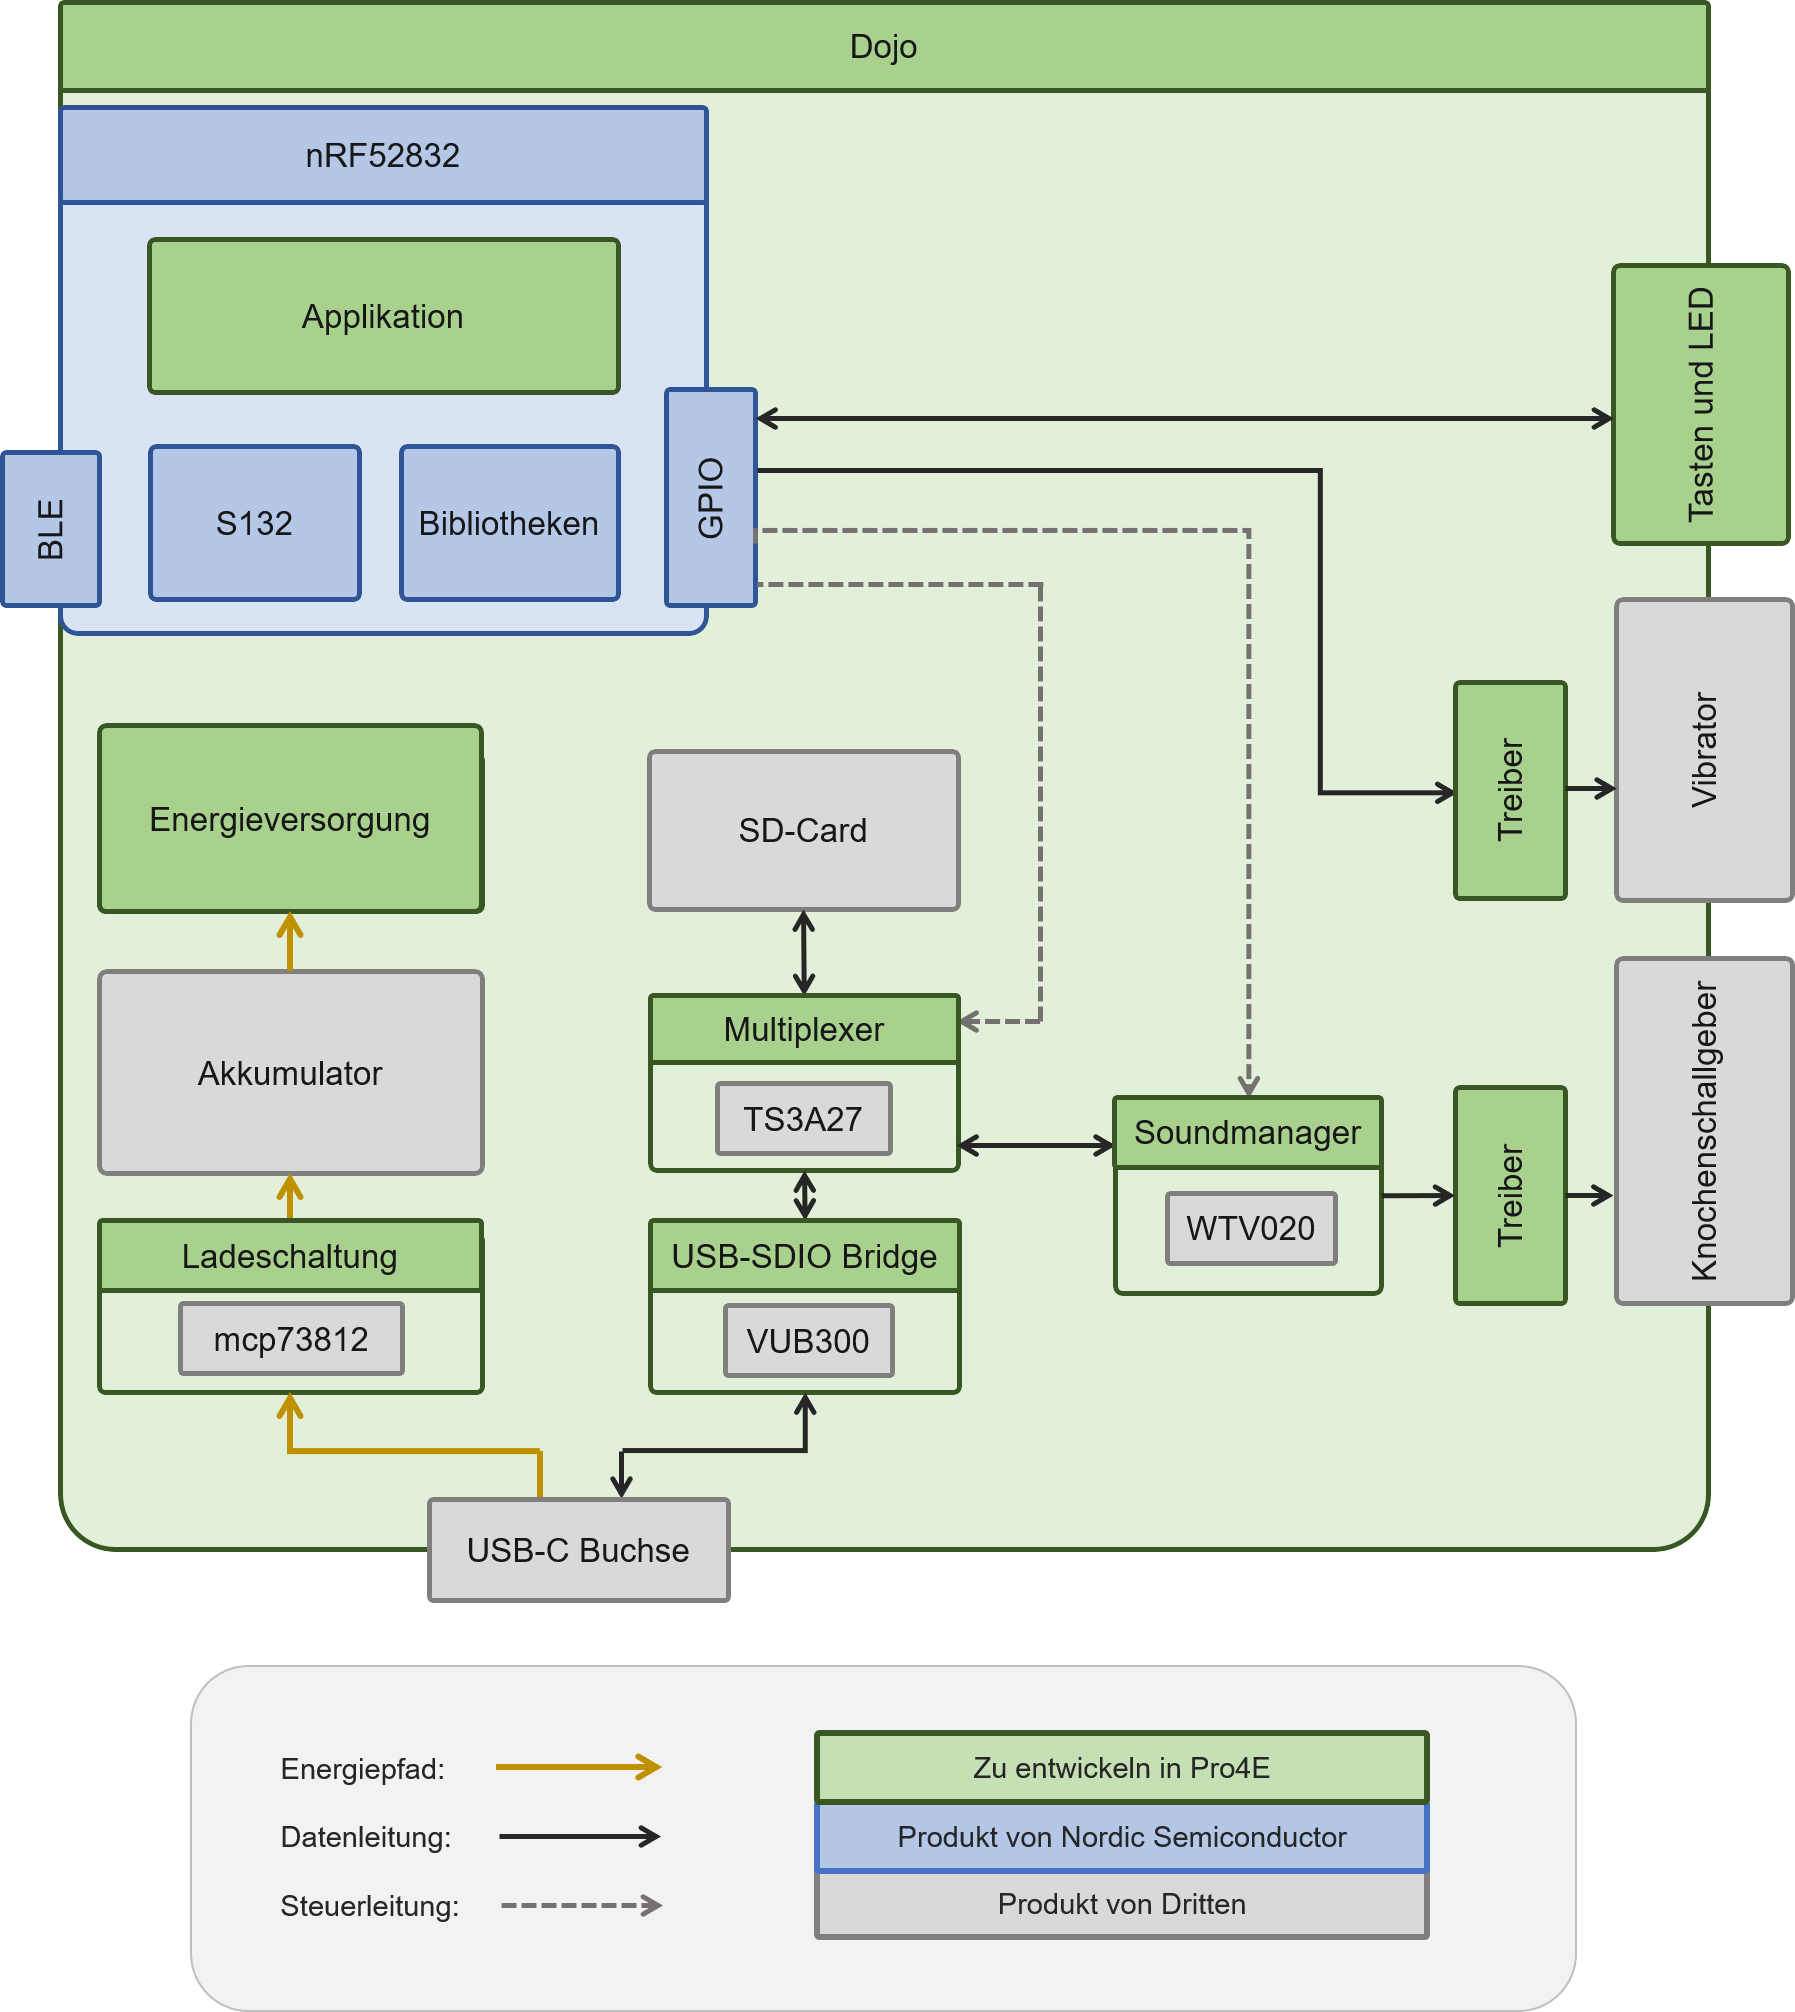
\includegraphics[width=0.8\textwidth]{graphics/Dojo.png}
    \caption{Hardwarekonzept des Dojo}
    \label{fig:HWKonzept}
  \end{figure}

\newpage
\subsection{Energieversorgung} \label{sec:Energie}
Die Elektronik des Dojos bezieht die Energie von einem Akkumulator. Verwendet wird ein Lithiumakkumulator der Marke Trustfire mit einer Nennspannung von $3.7V$. Der Akkumulator besitzt eine Ladungskapazität von $600mAh$.

\subsubsection{Entladevorgang} 
Der Akkumulator besitzt eine Nennspannung von $4.2V$ bei voller Kapazität und $0V$ \ref{test_Spannungsversorgung} wenn die Kapazität erschöpft ist. Die $0V$ kommen daher zustande, dass der Tiefenentladungsschutz der Batterie die Spannungsversorgung ab einer Spannung unter $2.75V$ kappt. Aus der Batteriespannung wird mit einem Linearregler des Types TL1963A eine $3.3V$ Spannungsversorgung erstellt. Mit dieser Versorgung wird die gesammte Elektronik gespiesen.

\subsubsection{Ladevorgang}
Der Akkumulator wird über die Spannungsversorgung des USB-Ports geladen. Ein Akkumulator-Management-Chip sorgt dabei für eine konstante Spannung von $4.2V$. Diese Spannung wird benötigt um den Akkumulator zu laden. Die Ladezeit beträgt $2.5h$, siehe Messungen Ladevorgang \ref{sec:Ladevorgang}. Somit ist es möglich, den Akkumulator über eine Nacht komplett zu laden, oder ihn zwischen den Benützungen einmal zu laden. 

\subsubsection{Messungen}
Um die Energieversorgung zu verifizieren wurden 3 verschiedene Messungen durchgeführt. Es wurde der Lade- und Entladevorgang aufgezeichnet, sowie die maximale mögliche Last ausgemessen.

\subsubsection*{Maximale Last}
Um herauszufinden welche Leistung bereitgestellt werden kann, wurde die Energieversorgung mit verschiedenen Lasten betrieben. 

\begin{table}[h]
\centering
\label{messungen_Energie}
\begin{tabular}{|l|c|c|c|}
\hline
Last [$\Omega$]     & 100   & 50    & 10    \\ \hline
Batteriestrom [$mA$]    & 32.55 & 63.79 & 293.3 \\ \hline
Batteriespannung [$V$] & 3.823 & 3.735 & 2.979 \\ \hline
Laststrom [$mA$] & 31.06 & 62.03 & 278.1 \\ \hline
Lastspannung [$V$]  & 3.293 & 3.292 & 2.95  \\ \hline
Leistung [$W$]  & 0.124 & 0.238 & 0.874  \\ \hline
\end{tabular}
\caption{Messungen mit verschiedene Widerstände}
\end{table}

Diese Daten zeigen, dass mit einer Leistung von $1W$ die Versorgungsspannung des Printes lediglich auf $2.95V$ sinkt. Dies entspricht einem Spannungsverlust von  $0.35V$, was in der Tolleranz aller elektronischen Bauteile liegt. Da auf unserem Print die maximale Last nur zwischen $0.3 - 0.5W$ liegt, treten keinerlei Probleme auf.
\newpage


\subsubsection*{Entladevorgang}
Um die Batterie zu entladen wurden 2 Messvorgänge durchgeführt. Beim ersten Messvorgang wurde eine Last von $30\Omega$ angeschlossen. Diese Last entspricht einem konstanten Entlagestom von $100mA$, was dem Stromverbrauch unserer Schaltung während dem Abspielen der Musik entspricht. Beim zweiten Messvorgang wurde eine Last von $220\Omega$ angeschlossen, welche einen konstanten Entlagestrom von $15mA$ ergibt. Dieser Entladestrom entspricht dem Verbrauch des Dojos im Ruhestatus. Die Messungen wurde bis zur vollständigen Entladung vollzogen. 
In den Abbildungen \ref{fig:SpannungZuZeit} und  \ref{fig:SpannungZuLadung} ist die Entladekurve für die Spannung im Vergleich zur Zeit und zur Ladung abgebildet:

\begin{figure}[h]
	 \subfigure[Entladekurve bei $100mA$ Entladestrom]{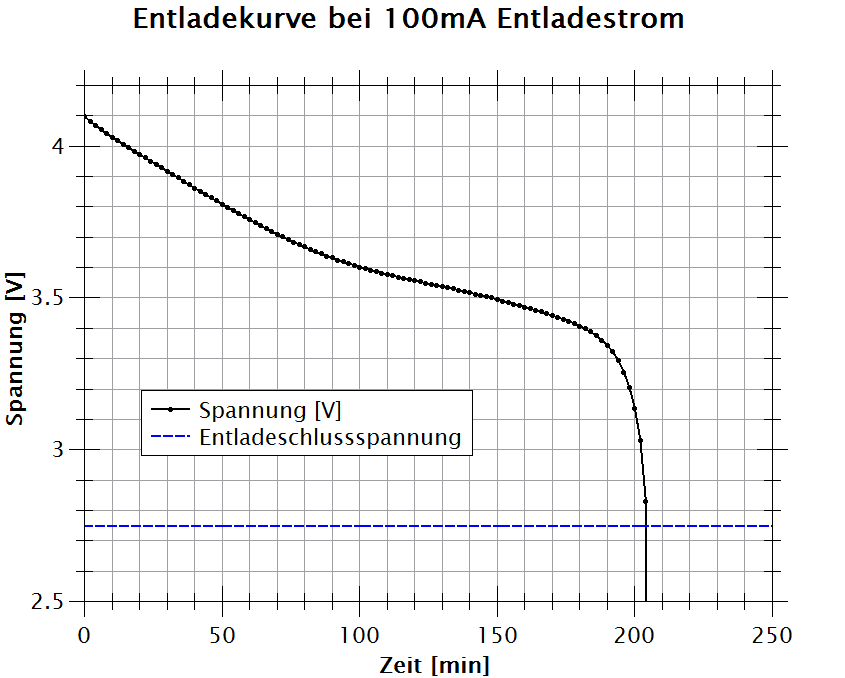
\includegraphics[width=0.49\textwidth]{graphics/SpannungzuZeit}} 
    \subfigure[Entladekurve bei $15mA$ Entladestrom]{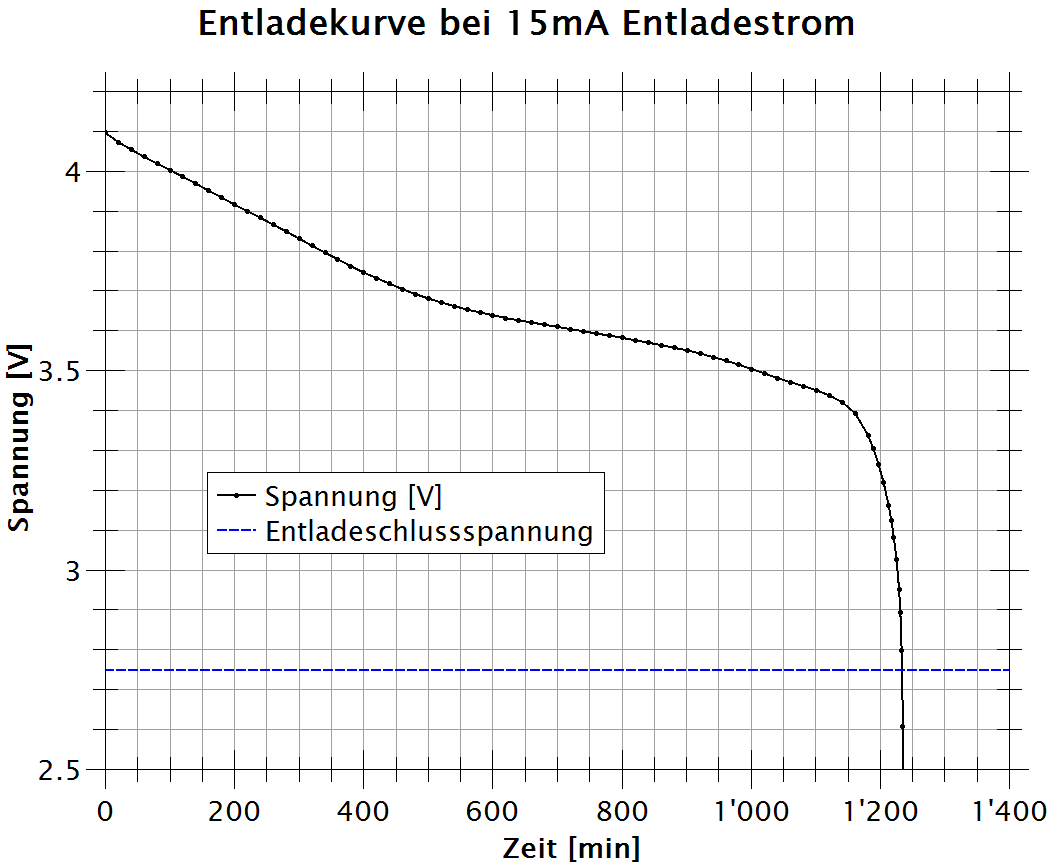
\includegraphics[width=0.49\textwidth]{graphics/SpannungzuZeit15}}
	\caption{Entladekurve der Batterie in Funktion der Zeit}
	\label{fig:SpannungZuZeit}
\end{figure}

Wie in der Abbildung \ref{fig:SpannungZuZeit} ersichtlich, hat die Batterie ein Tiefenentladungsschutz bei $2.75V$. Sobald diese Spannung erreicht ist, wird die Spannungsversorgung gekappt, und die Spannung sinkt auf $0V$.\\
Die gesammte Entladung dauert $3h 26min$ bei einem Entladestrom von $100mA$ und $20h50min$ bei einem Entladestrom von 15mA. Die effektive Laufzeit des Dojos befindet sich zwischen diesen Werten. Sie ist abhängig davo, wie stark der Dojo belastet wird, dass heisst, in welchem zyklus neue Audiofiles gestartet werden, und wie lange diese dauern.

\newpage

\begin{figure}[h]
	\centering
	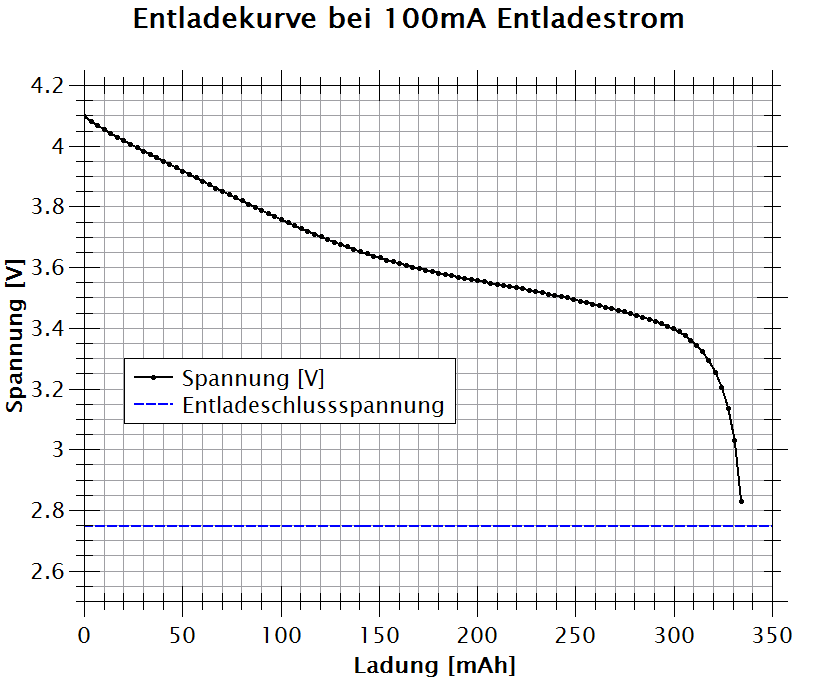
\includegraphics[width=\textwidth]{graphics/SpannungzuLadung.png}
	\caption{Spannung im Verhältnis zur Ladung. Bei einem Widerstand von 30$\Omega$}
	\label{fig:SpannungZuLadung}
\end{figure}

Die Abbildung \ref{fig:SpannungZuLadung} zeigt die abgegebene Ladung im Vergleich zur Batteriespannung. Sie zeigt, dass bei einer Belastung von 100mA und bei einer Belastung von 15mA die Ladung der Batterie im Schnitt $335mAh$ beträgt. Dies entspricht nicht der angegebenen Ladungskapazität von 600mAh, die der Hersteller verspricht. Die Messung zeigt uns, das der Hersteller die Angaben zu optimistisch ermittelt hat. Die Messung zeigt uns auch, dass die benötigte Spannung von $3.3V$ lange gehalten werden kann und erst bei einem Bezug von $320mAh$ die Spannung zusammenfällt.

\newpage

\subsubsection*{Ladevorgang}
\label{sec:Ladevorgang}
Beim Aufladen der Batterie wurde eine Spannung von $5V$ verwendet. Dabei wurde vor dem Anschliessen der Batterie ein Strom von $1.25mA$ gemessen. Die Ladekurve ist in der Abbildung                       \ref{fig:Ladeleistung} ersichtlich.

\begin{figure}[h]
	\centering
	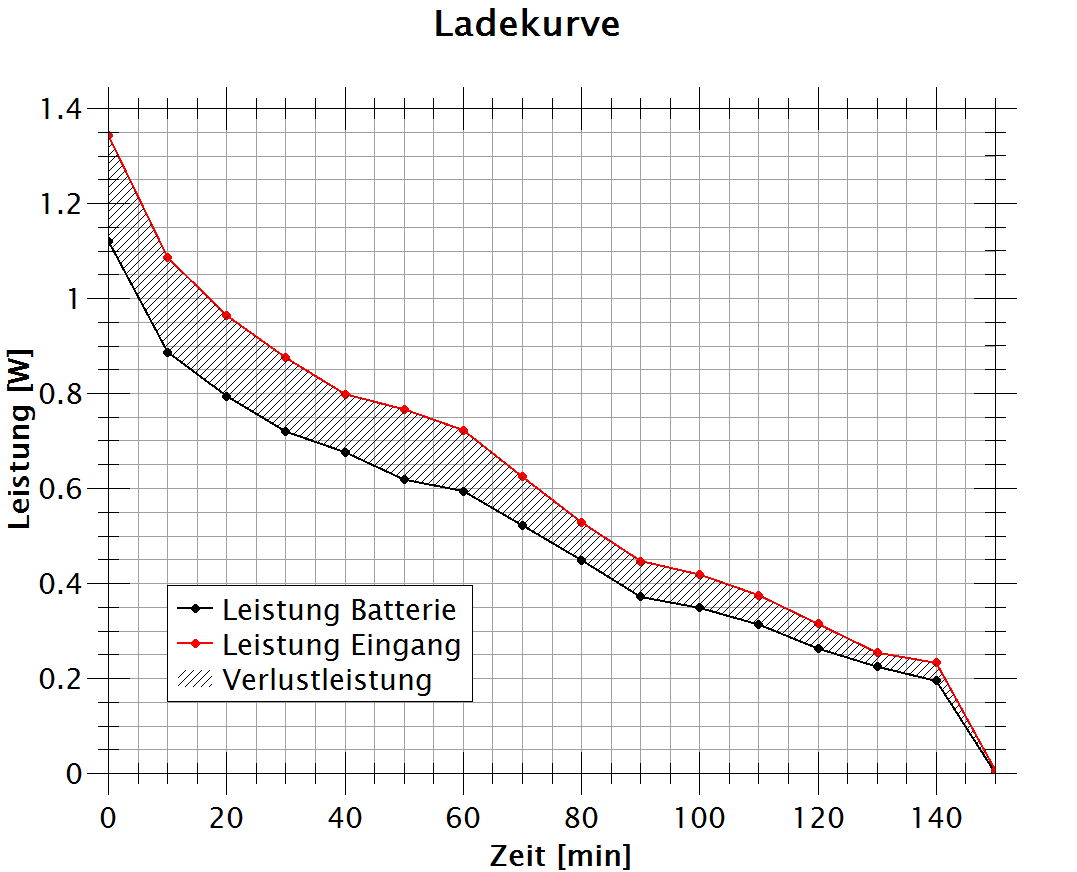
\includegraphics[width=\textwidth]{graphics/ladekurve.png}
	\caption{Ladekurve bei einer konstanten Eingangspannung von 5V}
	\label{fig:Ladeleistung}
\end{figure}

Die gestrichelte Fläche repräsentiert die Verlustleistung der Ladeschaltung beim Laden des Dojos.
Wir erhalten einen Wirkunsggrad von
\begin{equation}
\eta = 83.39%
\end{equation}
Das komplette Aufladen der Batterie dauerte $2.5h$. Somit kann das Museum den Dojo über Nacht problemlos aufladen. Auch Aufladungen zwischen Besuchen können so realisiert werden.
\clearpage



\subsection{Audio-Schnittstelle}\label{sec:AUDIO}

  Um den Entwicklungsaufwand zu begrenzen, wird ein Soundmanager-Chip implementiert, welcher selbständig aus einer Speicherkarte Audiodaten auslesen und wiedergeben kann. Verwendet wurde der WTV020, welcher über einen differentiellen Ausgang (zwei Anschlüsse) verfügt, an welchem direkt ein Lautsprecher angeschlossen werden könnte. 
  Im Datenblatt des WTV020 wird leider nicht definiert, welche Dimensionen der Ausgangstreiber hat. 
  Versuche haben jedoch gezeigt, dass die Leistung nicht ausreicht, um mit dem verwendeten Knochenschallgeber ein deutliches Audiosignal zu erzeugen. 
  Deshalb wird eine Treiberstufe in die Schaltung implementiert. 
  Diese hat die Aufgabe das differentielles Analogsignal vom WTV020 genügend niederohmig zur Verfügung zu stellen. 
  Für die Auswahl eines Treiberbausteins muss man deshalb die (frequenzabhängige) Impedanz des Knochenschallgebers kennen. 
  In der Abbildung \ref{fig:bode_knochenschall1} ist der mittels eines Frequenz Analysator (Agilent 4294A PRECISION IMPEDANCE ANALYZER) gemessene Impedanzgang des Knochenschallgebers dargestellt. 
  Der Impedanzgang in der linken Abbildung wurde mit einem frei in der Luft hängenden Knochenschallgeber gemessen. Man erkennt ein Resonanzverhalten bei ca. 2kHz. 
  Für die Messung in der rechten Abbildung wurde derselbe Knochenschallgeber verwendet, jedoch flach auf einen Tisch gelegt. 
  Dadurch verschwindet offenbar die zuvor erwähnte Resonanz. 
  Wie man auf den Abbildungen erkennen kann, befindet sich die Impedanz in einem Bereich über 4\(\Omega\) wird mit steigender Frequenz höher. 
  
  
  Die Treiberstufe muss Lasten von bis zu 4\(\Omega\) treiben können. 
  Es gibt diverse Audiotreiberbausteine, welche diese Aufgabe übernehmen können. 
  Diese Verstärker lassen sich in eine Hand voll Klassen aufteilen, welche sich von einander in der Art ihrer Ausgangsstufe unterscheiden. 
  Selbstverständliche bietet jede Klasse gewisse Vor- und Nachteile. 
  Verwendet man einen Klasse-A-Verstärker, erreicht an am wenigsten Signalverzerrung auf Kosten des Energieverbrauchs. 
  Ein Klasse-D-Verstärker hingegen ermöglicht einen sehr effizienten Betrieb, verzehrt dafür das Signal stärker. 
  Für dieses Projekt wurde Wiedergabe von Sprache und Musik mit diesen beiden Typen getestet (Klasse-A: TS4871 von STMicroelectronics und Klasse-D: PAM8302AASCR von Diodes Incorperated). 
  Subjektiv betrachtet, waren beide Typen in der Lage, Audiodaten in einer sinnvollen Qualität wiederzugeben und man konnte keinen Qualitätsunterschied feststellen. Der Energieverbrauch des Klasse-A-Verstärkers (ca. 120mA) war jedoch rund 6 mal höher als derjenige des Klasse-D-Verstärkers (20mA).
  Dieses Resultat wurde so erwartet. Weil der Klasse-A-Verstärker keinen merklichen Vorteil bot, wurde der PAM8302AASCR in die Elektronik implementiert.
  
  \begin{figure}[h]
	 \subfigure[Bei 2kHz kann eine Resonanz beobachtet werden.]{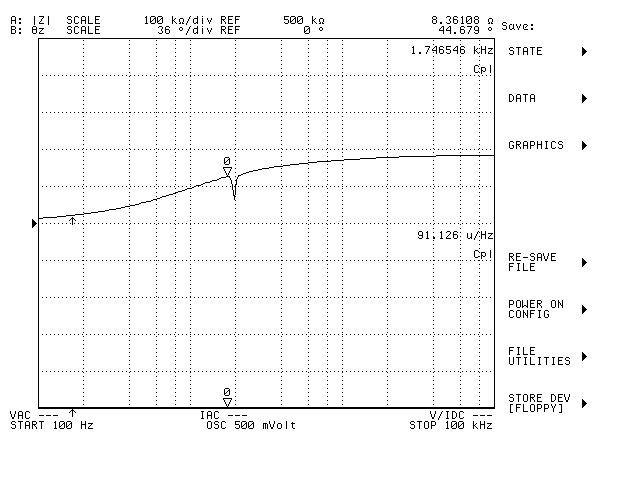
\includegraphics[width=0.49\textwidth]{graphics/123111.png}} 
    \subfigure[Die Resonanz bei 2kHz ist nicht vorhanden.]{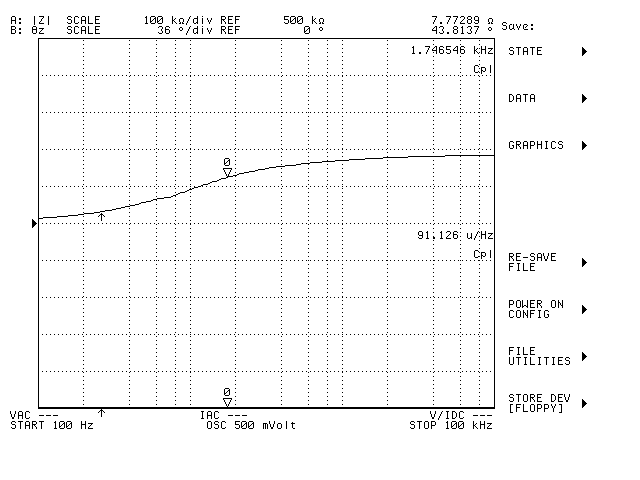
\includegraphics[width=0.49\textwidth]{graphics/123222.png}}
	\caption{Bodediagramm Knochenschallgeber}
	\label{fig:bode_knochenschall1}
  \end{figure}
  
  
  \clearpage
  
  \subsubsection{Versuch: Passive Anpassung der Last:}
  Es wurde versucht ein simples Ersatzschaltbild für das elektrische Verhalten des Knochenschallgebers zu finden. 
  Das Ziel war, mit einer passiven Schaltung die Impedanz von diesem auf den Ausgang des Soundmanger-Chips oder einer Treiberstufe anzupassen. 
  Als elektrisches Modell für den Knochenschallgeber wurde eine RL-Serienschaltung gewählt. 
  Mit einem Impedanzmessgerät (PM 6303 RCLmeter von der Ingenieurschule beider Basel in Muttenz) wurde die serielle Induktivität und der serielle Widerstand bei f=1000Hz an einem Knochenschallgeber gemessen und in Matlab (siehe Anhang \ref{fig:matlab_anhang}) wurde der Impedanzgang des Modells analysiert (siehe Abbildung \ref{fig:Impedanz_Knochenschall_modell}). 
  Man kam zu der Erkenntnis, dass mittels einer seriellen Kapazität einerseits der effektive Strom durch den Knochenschallgeber (im Frequenzbereich der Sprache) erhöht werden kann und ausserdem tiefe Frequenzen weg gefiltert werden. 
  Letzteres hat den Vorteil, dass die Impedanz der Lastschaltung bei Tiefen Frequenzen nicht unter ca. 8\(\Omega\) fallen würde. Da Versuche mit dem WTV020 gezeigt haben, dass dieser bei Frequenzen über 1000Hz in der Lage ist eine 4\(\Omega\) Last zu treiben,
   könnte man damit evtl. auf einen separaten Treiberbaustein in der Schaltung verzichten. 
  Die menschliche Sprache würde weiterhin verständlich sein, da unser Gehirn allen, durch die Schaltung weg gefilterten, Grundschwingungen aus dessen Oberschwingungen zusammensetzen kann. 
  Versuche haben jedoch gezeigt, dass tiefe Stimmen nur leise wahrgenommen werden. 
  Aus diesem Grund wurde der Ansatz mit der passiven Schaltung verworfen und man entschied sich definitiv dafür eine separate Treiberstufe zu verwenden, welche eine niederohmige Last treiben kann.
  
  \begin{figure}[h]
	\centering
	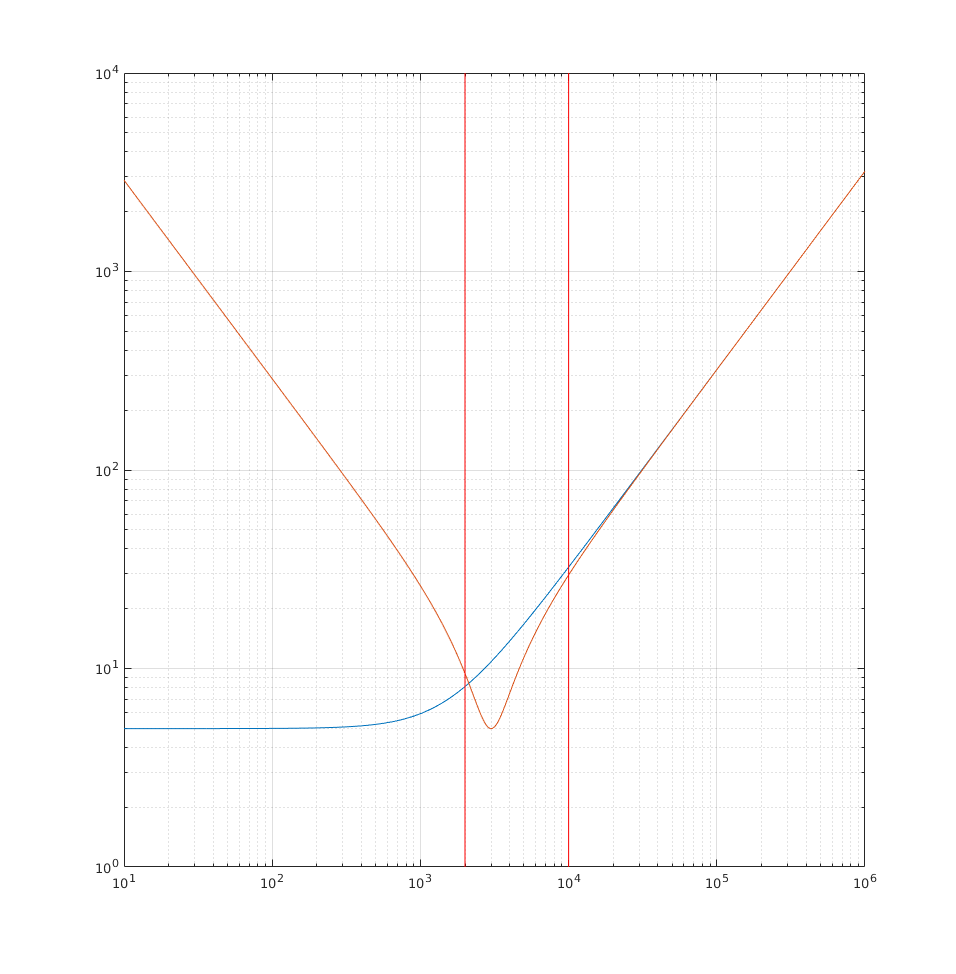
\includegraphics[width=0.72\textwidth]{graphics/RLGlied.png}
	\caption{Dargestellt ist der Impedanzverlauf des Knochenschallgebers ohne Anpassnetzwerk (blaue Kurve) und mit Anpassnetzwerk (orange Kurve). Die beiden roten Striche zeigen den für Sprache besonders wichtigen Bereich zwischen 2kHz und 10kHz.
	Wie man erkennen kann, verhindert das externe Anpassnetzwerk einerseits, dass die Impedanz des Knochenschallgebers bei unter 1000Hz unter 8\(\Omega\) fällt und senkt die Impedanz im relevanten Bereich. Letzteres erhöht die Lautstärke.}
	\label{fig:Impedanz_Knochenschall_modell}
  \end{figure}
  
  



\subsection{USB-Schnittstelle}\label{sec:USB}
Das Konzept im Pflichtenheft sieht vor, dass ein Computer auf eine Speicherkarte auf dem Dojo wie auf ein Laufwerk zugreift. Gewöhnlich löst man dieses Problem indem man einen Mikrocontroller mit USB-Peripherie in die Elektronik implementiert.
Dieser Mikrocontroller müsste dann ausserdem mit einem komplexen Speichersystem arbeiten können. Um dieses Problem zu umgehen, wird in diesem Projekt die USB/SDIO-Bridge VUB300 von Elan verwendet. Diese verwaltet selbständig die Kommunikation zwischen dem PC und der SD-Karte.
Der VUB300 unterstützt USB2.0 High-Speed. 

\vspace{0.2cm}

\paragraph{Achtung:} Leider funktioniert der Zugriff auf Speicherkarten nur bei bestimmten Karten. 
Welche Karten sich eigenen ist unklar, da kein Muster betreffend Format, Grösse oder Alter erkannt werden konnte.
Ausserdem existiert kein Treiber für Windows 8 oder neuer, weshalb für den hier entwickelten Dojo Linux oder ein altes Windows verwendet werden muss.
Weiterhin existiert die Herstellerfirma Elan nach unseren Erkenntnissen nicht mehr. Aus diesen Gründen wird bei einer allfälligen Weiterentwicklung des Produktes stark davon abgeraten den VUB300 weiterhin zu verwenden.
Stattdessen wird empfohlen den Nachfolger von verwendeten Mikrocontroller zu verwenden. Dieser (nRF52840) bietet eine USB-Peripherie und ist fähig auf eine Speicherkarte zuzugreifen. 

\subsection{Zugriff auf SD-Karte}\label{sec:SD_KART}
Auf die SD-Karte greifen sowohl der VUB300 als auch der WTV020 zu. Da nicht beide Komponenten gleichzeitig auf die SD-Karte zugreifen können muss ein Multiplexer verwendet werden, mit welchem der Mikrocontroller je nach Situation den Zugriff regeln kann.
An diesen sind aufgrund des schnellen SDIO-Busses hohe Anforderungen gestellt. Die bis zu 50MHz schnellen Signale müssen ohne zu grosse Verzehrung durch den Multiplexer geleitet werden. Der Multiplexer TS3A27 wird diesen Anforderungen gerecht.
Erwähnenswert ist noch, dass auch die Spannungsversorgung der SD-Karte gesteuert werden muss, da sie vom VUB300 zum zurücksetzen benutzt wird. Da der verwendete Multiplexer keinen Kanal für die Spannungsversorgung frei hat, wurde eine kleine Logikschaltung (D1, T1 und T2) entwickelt, welche diese Aufgabe übernimmt (siehe Tabelle \ref{tab:zugriff}).
Bei den verwendeten Transistoren muss darauf geachtet werden, dass der Durchlasswiderstand klein ist (\(<1\Omega\)). Ausserdem wird parallel zur SD-Karte ein Stützkondensator eingefügt. Dieser verhindert Spannungseinbrüche beim Betrieb.

\vspace{1cm}

\begin{table}[h]
  \centering
  \begin{tabular}{|c|c|c|}
    \hline
    /EN & IN & POWER\\
    \hline
    0 & 0 & VUB300 PWR PIN \\
    \hline
    0 & 1 & ON \\
    \hline
    1 & 0 & OFF \\
    \hline
    1 & 1 & OFF \\
    \hline
  \end{tabular}
  \caption{Logiktabelle zum SD-Karten zugriff}\label{tab:zugriff}
\end{table}
 
\newpage

\subsection{Zum Layout}
    Verschiedene PDF's zum Layout befinden sich im Anhang \ref{}.
    Die Leiterplatte ist im Formfaktor des Dojo ( \( (17\times 115)mm \) ) und beinhaltet vier Lagen. 
    Alle Durchkontaktierungen sind vom Typ through hole. 
    Der minimale Kupferabstand beträgt 0.15mm und der minimale Bohrdurchmesser beträgt 0.3mm.
    Die beiden inneren Lagen beinhaltet beide eine durchgehende Kupferfläche. 
    Einmal auf Ground und einmal auf VCC.
    Alle sonstigen Verbindungen befinden sich auf den Aussenlagen des Prints.
    Zwecks Bestückung im Lötofen befinden sich fast alle Bauteile auf der selben Seite. 
    Nur die Tasten, LED's, der Programmierstecker und die USB-Buchse befinden sich auf der Oberseite.
    Auf vorderen Seite der Leiterplatte befindet sich der Energieversorgungsteil. 
    Um hier entstehende Wärme abzuleiten, wurde hier auch auf einer Aussenlage eine Kupferfläche eingefügt.
    Der Mikrocontroller (nRF52) wurde nicht direkt auf die Leiterplatte implementiert, sondern es wurde ein ASIC verwendet, welcher die 2.4GHz Antenne beinhaltet.
    Im Datenblatt dieses ASIC (ISP1507) wird empfohlen unterhalb der Antenne auf Kupferflächen zu verzichten, was so befolgt wurde.
    Die USB-Verbindungen wurde bewusst Kurz und die Leitungen gleich lang eingeplant. 
    Aus diesem Grund befindet sich die USB-Buchse auf der Oberseite des Prints (um ein Kreuzen der Datenleitungen zu vermeiden) und der USB-Teil befindet sich am hinteren Teil des Dojos.
    Auch der SDIO-Bus, der vom VUB300 über den Multiplexer zur SD-Karte verläuft wurde möglichst kurz gelayoutet. 
    Im Datenblatt vom VUB300 werden für jeden Spannungsversorgungspin zwei Kondensatoren (1\(\mu F\) und 100\(nF\)) vorgeschlagen. 
    Diese Praxis ist jedoch wenig sinnvoll, wenn beide Kondensatoren in einem gleich grossen Gehäuse erhältlich sind.
    Aus diesem Grund wurde nur jeweils ein 100\(nF\) Kondensator implementiert. 
    
    \vspace{0.2cm}
    
    \paragraph{Achtung:} Beim Layouten wurde eine Verbindung nicht umgesetzt. Es handelt sich um die Standby-Leitung des Audioverstärkers, mit welcher der Mikrocontroller diesen in den Standby-Zustand versetzen kann.
    Auf der aktuellen Version der Leiterplatte wird der betroffene Pin mit einer Drahtbrücke konstant auf VCC gezogen. 
    Dies ist vertretbar, da der Stromverbrauch des Audioverstärkers ohne Audiosignal nicht ins Gewicht fällt.
    
\subsection{Zu den Tasten}
    Die Tasten werden per Software entprellt. 
    Die verwendete Button-Bibliothek von Nordic sollte dazu in der Lage sein, doch leider prellen die verwendeten Tasten zu lang und es kommt immer wieder zu Fehlinterpretationen. 
    Um das Problem zu beheben, wurde bei jeder Taste ein \(10\mu F\) Kondensator parallel angeschlossen. Dadurch wurde konnte das Prellen genug stark unterdrückt werden und die Eingabe funktioniert nun ohne Prellen.
    Die erwähnten Kondensatoren sind auf dem Schema nicht ersichtlich.
    
   
\newpage
  